% !TeX spellcheck = en_US
\documentclass[11pt, a4paper]{article}
\usepackage[utf8]{inputenc}
\usepackage[toc,page]{appendix}

\usepackage{latexsym}
\usepackage{float}
\usepackage[utf8]{inputenc}
\usepackage[english]{babel}
\usepackage{microtype}
\usepackage[hyphens]{url}
\usepackage{hyperref}
\usepackage{graphicx}
\usepackage[nonumberlist,acronym]{glossaries}
\usepackage{makeidx}
\usepackage{dsfont}
\usepackage{datetime}
\usepackage{multicol}
\usepackage{setspace}
\usepackage{pdflscape}
\usepackage{pgffor}
\usepackage{enumerate}
\usepackage{booktabs}
\usepackage{tabularx}
\usepackage{braket}
\usepackage{listings}
\usepackage{color}
\usepackage{amsmath}
\usepackage{amssymb}
\usepackage[table,xcdraw]{xcolor}
\usepackage{graphicx}
\usepackage{listings}
\usepackage{hyperref}
\usepackage{vmargin}
\usepackage{changepage}
\usepackage{wrapfig}
\usepackage{subfiles}
\usepackage{float}
\usepackage{amsmath}
\usepackage{amssymb}
\usepackage{tikz-cd}
\usepackage{multirow}
\usepackage{pgffor}
\usepackage{enumitem}
\usepackage{iflang}
\usepackage{varioref}
\usepackage{hyperref}
\usepackage{cleveref}
\usepackage[justification=centering]{caption}
\usepackage{subcaption}
\usepackage{tikz}
\usepackage{enumitem}
\usepackage{xpatch}
\usepackage{refcount}
\usepackage{color}
\usepackage{pdfpages}
\usepackage{array}
\usepackage{eurosym}
\usetikzlibrary{mindmap}

%%%%%%%%%%%%%%%%%%%%%%%%%%%%%%%%%%%%%%%
%%%%%%%%%%%% UTIL COMMANDS %%%%%%%%%%%%  

\setcounter{secnumdepth}{4}
\newcommand{\nc}{\newcommand}
\nc{\supindex}{\textsuperscript}
\renewcommand{\baselinestretch}{1.5}
\nc{\myparagraph}[1]{\paragraph{#1}\mbox{}\\}

%%%%%%%%%%%%%%%%%%%%%%%%%%%%%%%%%%%%%%%
%%%%%%%%%%%%% CONFIG FILE %%%%%%%%%%%%%

\nc{\mytitle}{Generative deep learning based models for cloud removal satellite imagery}
\nc{\mysubtitle}{Bayesian Inference}
\nc{\authors}{\textit{Oriol Alàs Cercós}}
\nc{\datetime}{25\supindex{th} of May, 2022}
\nc{\assignatura}{Technological Business Management and Entrepreneurship}
\nc{\professorat}{Josep Escribà Garriga}

% Per separar professors, utilitzar ','
% 	Ex: Maria, Joan, Pere

%%%%%%%%%%%%%%%%%%%%%%%%%%%%%%%%%%%%%%%
%%%%%%%%%%%%%  LANGUAGE   %%%%%%%%%%%%%

\newcommand{\tr}{\IfLanguageName{english}}

%%%%%%%%%%%%%%%%%%%%%%%%%%%%%%%%%%%%%%%
%%%%%%%%%%%%%%%%% MATH %%%%%%%%%%%%%%%%

\nc{\prob}[1]{P({#1})}
\nc{\probl}[2]{P({#1}|{#2})}

%%%%%%%%%%%%%%%%%%%%%%%%%%%%%%%%%%%%%%%
%%%%%%%%%%%%% FUNCTIONS %%%%%%%%%%%%

\nc{\numitems}[1]{\getrefnumber{#1}}
\newcounter{itemcntr}
\AtBeginEnvironment{itemize}{%
	\setcounter{itemcntr}{0}%
	\xapptocmd{\item}{\refstepcounter{itemcntr}}{}{}%
}

%%%%%%%%%%%%%%%%%%%%%%%%%%%%%%%%%%%%%%%
%%%%%%%%%%%%% RADIO BUTTON %%%%%%%%%%%%

\makeatletter
\newcommand*{\radiobutton}{%
	\@ifstar{\@radiobutton0}{\@radiobutton1}%
}
\newcommand*{\@radiobutton}[1]{%
	\begin{tikzpicture}
		\pgfmathsetlengthmacro\radius{height("X")/2}
		\draw[radius=\radius] circle;
		\ifcase#1 \fill[radius=.6*\radius] circle;\fi
	\end{tikzpicture}%
}
\makeatother


%%%%%%%%%%%%%%%%%%%%%%%%%%%%%%%%%%%%%%%
%%%%%%%%%%%%%  %%%%%%%%%%%%


\newcolumntype{S}{>{\centering\arraybackslash}m{1.5em}}

\renewcommand{\tabularxcolumn}[1]{m{#1}} % redefine 'X' to use 'm'
\newcommand{ \titem}[1]{\item \textbf{#1}\quad}


\newcolumntype{P}[1]{>{\centering\arraybackslash}p{#1}}

\setpapersize{A4}

\author{Oriol Alàs Cercós}
\date{29 d'Abril del 2019}

\makeglossaries
\newacronym{rs}{RS}{Remote Sensing}
\newacronym{sar}{SAR}{Synthetic Aperture Radar}
\newacronym{cnn}{CNN}{Convolutional Neural Network}
\newacronym{mlp}{MLP}{Multi-Layer Perceptron}
\newacronym{gan}{GAN}{Generative Adversarial Network}
\newacronym{cgan}{cGAN}{Conditional Generative Adversarial Network}
\newacronym{mcgan}{McGAN}{Multi-spectral Conditional Generative Adversarial Network}
\newacronym{nir}{NIR}{Near Infra Red}
\newacronym{ir}{IR}{Infra Red}
\newacronym{l1c}{L1C}{Level-1C}
\newacronym{l2a}{L2A}{Level-2A}
\newacronym{nlp}{NLP}{Natural Language Processing}
\newacronym{psnr}{PSNR}{Peak signal-to-noise ratio}
\newacronym{ssim}{SSIM}{Structural Similarity Index Metric}
\newacronym{rnn}{RNN}{Recurrent Neural Network}
\newacronym{vit}{ViT}{Vision Transformer}
\newacronym{ltae}{L-TAE}{Lightweight Temporal Attention Encoder}
\newacronym{tae}{TAE}{Temporal Attention Encoder}
\newacronym{vae}{VAE}{Variational AutoEncoder}
\newacronym{bce}{BCE}{Binary Cross Entropy}
\newacronym{ddm}{DDM}{Denoising Diffusion Model}
\newacronym{elbo}{ELBO}{Evidence Lower Bound}
\newacronym{kl}{KL}{Kullback-Leibler}
\newacronym{sam}{SAM}{Spectral Angle Mapper}
\newacronym{mse}{MSE}{Mean Squared Error}
\newacronym{mae}{MAE}{Mean Absolute Error}
\newacronym{carl}{CARL}{Cloud-Adaptive Regularized Loss}
\newacronym{eda}{EDA}{Exploratory Data Analysis}
\newacronym{kde}{KDE}{Kernel Density Estimation}
\newacronym{relu}{ReLU}{Rectified Lineal Unit}

\def\contentsname{Índex}
\begin{document}
	
	\definecolor{gray}{rgb}{0.4,0.4,0.4}
	\definecolor{darkblue}{rgb}{0.0,0.0,0.6}
	\definecolor{cyan}{rgb}{0.0,0.6,0.6}
	\lstset{
		basicstyle=\ttfamily,
		columns=fullflexible,
		showstringspaces=false,
		commentstyle=\color{gray}\upshape
	}
	
	\lstdefinelanguage{XML}
	{
		morestring=[b]",
		morestring=[s]{>}{<},
		morecomment=[s]{<?}{?>},
		stringstyle=\color{black},
		identifierstyle=\color{darkblue},
		keywordstyle=\color{cyan},
		morekeywords={xmlns,version,type}% list your attributes here
	}
	
	\begin{titlepage}
		\begin{figure}[htb]
			\begin{center}
				
				\includegraphics[width=5cm]{imgs/udl.png}\\
				
				
				\medskip
				\begin{center}
					
					\huge\textbf{\mytitle}\\
					\bigskip
					\normalsize{\tr{Made by}{Realitzat per:}}
					\\
					\large\textit{\authors}
					\\
					\setlength{\parskip}{1em}
					\normalsize{\tr{Delivery}{Data de lliurament:}}
					\\
					\large{\datetime}
				\end{center}
				
				\vspace*{\stretch{2.0}}
			\end{center}
		\end{figure}
		\begin{flushright}
			Universitat de Lleida
			\\
			Escola Politècnica Superior
			\\
			Màster en Enginyeria Informàtica
			\\
			\assignatura
			\\
			\medskip
			\textbf{\tr{Professorate:}{Tutor:}}
			\\
			\foreach \n in \professorat{\n\\}
		\end{flushright}
		\thispagestyle{empty} 
	\end{titlepage}
	\pagenumbering{roman}
	\tableofcontents
	\newpage
	\listoffigures
	\newpage
	\listoftables
	\newpage
	\printglossary[type=\acronymtype]
	\newpage
	\pagenumbering{arabic}

	\part{Introduction} 
	\gls{rs} imagery is critical to overcome challenges such climate change or natural resources management, including zone monitoring for reforestation, disaster mapping, evolution, and impact assessment, land surface change detection and coastal water quality monitoring.  
	Nevertheless, on average 55\% of the Earth's land surfaces is covered by clouds, being then a significant impediment to carry out a broad range of applications. Satellite imagery plagued by films of clouds that obstructs the scene implies a great loss of information or causing effects such as blurring, which mitigates the power of \gls{rs}. Hence, \gls{rs} applications would be greatly improved with techniques aimed at detecting and removing cloudy regions, and proving in-painting capabilities for the underlying scene, thus allowing for better analytics and decision support.
	\\
	\\
	On the other hand, my interest in deep learning and computer vision has truly flourished over the past two years. During my initial project in computer vision focused on satellite images, I suffered hard times because of cloud coverage. Regrettably, many ideas couldn't be realized without access to a dependable weekly record that would meet the end user's reliability requirements. This experience has piqued my curiosity for tackling new challenges and, most importantly, learning from them to pave the way for future endeavors. 
	\\
	\\
	Furthermore, deep learning has, in recent years, unveiled opportunities that were entirely unimaginable just a decade or two ago. Its immense potential, especially in generative models, holds the promise of substantial societal and environmental advancements. However, grasping the intricacies of these models and determining when to employ one over the other can prove rather challenging without a dedicated period of learning and experimentation. 
	\\
	\\
	In this ever evolving landscape, the intersection of \gls{rs} and deep learning holds the promise of advancing our understanding of the world and our ability to tackle complex global issues. So why not embark on this journey?
	\newpage
	\section*{Objectives}
	Once set the challenge and the motivation, the goals of this master thesis are:
	\begin{itemize}
		\item Search state-of-the-art approaches as well as frameworks that could bring new improvements and better results.
		\item Create or search for a multi-temporal and spatial imagery to design and evaluate a model that can remove the clouds given a satellite image.
		\item Design and implement an effective model and monitoring its training.
		\item Evaluate the model and provide a benchmark with other approaches.
	\end{itemize}
	\newpage
	\section*{Task planification}
	Creating a project plan and establishing timelines for each task are essential steps in effectively managing your deep learning project. To ensure efficient project management and maintain a consistent work pace, the project has been broken down into three main tasks, each further subdivided into smaller components. These tasks include:
	\begin{itemize}
	\item \textbf{Study of the problem and review of the State of the Art}. This task involves conducting a comprehensive analysis of the problem the project aims to solve. It not only includes a detailed examination of existing research and methodologies relevant to the problem but also comprehends the technical requirements to do the following tasks.
	\item \textbf{Data exploration}. Data exploration entails the thorough investigation of the dataset or datasets to be used in the project. This process includes data collection, cleaning, preprocessing, and augmentation as necessary. The goal is to understand the data's characteristics
	\item \textbf{Training and generation of sample results}. The training and generation of sample results constitute the practical implementation phase of the project. This step also involves hyperparameter tuning and iterative model improvements. Ultimately, the goal is to generate sample results that demonstrate the model's ability to remove clouds from satellite images, showcasing the effectiveness of the developed algorithms.
	\end{itemize}
	\begin{figure}[H]
		\caption{Project timeline}
		\centering
			\begin{adjustwidth}{-2cm}{}
		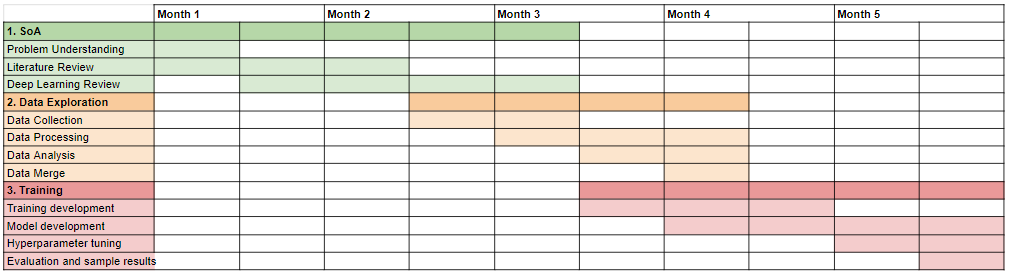
\includegraphics[width=18cm]{imgs/gantt.png}
		\end{adjustwidth}
	\end{figure}
	\newpage
	\section{Problem Analysis}
	\gls{rs} is a scientific method used to obtain information about objects or areas from a distance, typically from aircraft or satellites. This technique involves detecting and measuring the radiation that is emitted or reflected by these objects or areas. Remote sensing is widely used in various fields such as meteorology, agriculture, geology, and environmental science, among others.
	\\
	\\
	Traditional ground-based data collection methods can be resource-intensive, requiring transportation, equipment, and personnel. In this way, \gls{rnn} minimizes the need for these, conserving resources. Satellite-based observations reduce the need for on-ground surveys, which can involve vehicles and equipment that emit greenhouse gases. When cloud interference is removed, satellite imagery provides a more comprehensive view of large areas, ensuring that no critical changes or patterns are missed. Moreover, the timely access to clear images can be crucial for monitoring and responding to environmental changes or disasters.
	\\
	\\
	Although there are several constellations and a high diversity of aerial and satellite images, the problem has been focused using Copernicus Sentinel2 constellation. The reason why is simple, Sentinel constellation imagery is freely available to the public, making it accessible for researchers, scientists, and organizations around the world. Definitely, open data policy encourages innovation and the development of a wide range of applications.
	\subfile{sections/soa}
	\newpage
	\part{Development}
	\section{Exploratory Data Analysis}
	\subfile{sections/eda}
	\subsection{Data merge strategy}
	\subfile{sections/datamerge}
	\newpage
	\section{Model training}
	\subsection{Technologies}
	\subfile{sections/stack}
	\subsection{Losses and metrics}
	\subfile{sections/metrics}
	\subsection{Models architecture}
	\subfile{sections/models}
	\section{Experiments and results}
	\subfile{sections/results}
	\section*{Economic Analysis}
	While the project primarily centers around research, it's essential to consider that applied research incurs costs. Consequently, a basic economic analysis has been carried out to assess the expenses incurred thus far.\\
	\\
	In the economic analysis, we assumed that an individual with a master's degree would cost the company approximately 70€/h. Given that the work was conducted on a part-time basis, a total of 430 hours were spent, equating to 30100€. 
	On the other hand, the GPU was used for a total of 182 hours. Given that the average price is around €2 \cite{price-gpu} per hour, €364 was spent in total. Considering that machine learning or deep learning projects typically cost between 60000€ to 100000€, the project remains profitable. However, since there is job to be done the required time for the project would decrease its profitability. Assuming it will be needed one entire month more, the expenditure could amount to a total of €42,140.
	\begin{table}[H]
		\centering
		\caption{Cost of the project}
		\begin{tabular}{c|ccc}
		 & Value & Conversion & Total (\euro) \\\hline
		PM	& 2.5 PM & $70 \frac{\text{\euro}}{h}$ & $30100 €$ \\
		GPU	& 182 hours & $2 \frac{\text{\euro}}{h}$ & $364 €$ \\\hline
		Total & & & $30464 €$\\\hline\hline
		Predicted PM & 2.5 PM & $70 \frac{\text{\euro}}{h}$ & $12040 €$\\\hline
		Total & & & $42140 €$\\	
		\end{tabular}
	\end{table}
	
	%
	
	\newpage
	\part{Conclusions}
	In summary, the introduction and results suggest that while RS imagery and deep learning hold great promise, there is a need for more powerful neural networks, improved data normalization, and consideration of alternative approaches to overcome cloud coverage challenges.
	\\
	\\
	The project aimed to search for and analyze state-of-the-art approaches and frameworks in the field of remote sensing and deep learning. This exploration was intended to identify novel methods that could lead to improvements and superior results in cloud removal from satellite imagery.
	\\
	\\
	Technically, the project's cautious approach of using less powerful neural networks for methodical development has led to delays. There is a clear need to reconsider this approach and explore more potent neural network models to expedite progress. Some challenges were exacerbated by issues with data normalization. Recognizing these issues at a later stage hindered model learning and contributed to setbacks. Addressing normalization problems is crucial for better results. The project found that diffusion models were more time-consuming than initially suspected. This highlights the importance of careful consideration and optimization in the implementation of such models to make them computationally efficient.
	\\
	\\
	Professionally, I must admit that the Master's thesis has provided me with extensive knowledge about generative images. However, there is still a considerable distance to cover before I can feel entirely at ease with this type of problem-solving and approach it with greater ease. On the positive side, I now feel more capable and prepared to rigorously adhere to project timelines, even if it requires prioritizing certain aspects over others. This experience has taught me the importance of identifying what truly matters and having the ability to emphasize or de-emphasize elements based on their relevance to the project's ultimate goals. In essence, this project has been a valuable learning experience, helping me establish effective boundaries when working on complex tasks.
	
	\newpage
	\bibliography{bibliography}
	\bibliographystyle{unsrt}
	\newpage
	\subfile{sections/appendix.tex}
	
\end{document}
